\documentclass[a4paper]{article}

\usepackage{graphicx}
\usepackage{amsmath,amssymb}
\usepackage{minted}
\usepackage{multirow}
\usepackage{float}
\usepackage{algorithm}
\usepackage{algpseudocode}
\usepackage{todonotes}
\usepackage{forest}
\usepackage{xstring}
\usepackage{xcolor}
\usepackage[most]{tcolorbox}
\usepackage{xparse}
\usepackage{natbib}
\usepackage{adjustbox}

\usetikzlibrary{graphs,graphdrawing}
\usegdlibrary{layered}

% for external graphviz
\input{/home/donkarlo/Dropbox/repo/nd_language_ai_project/src/nd_language_ai/formal/computer/programming/tex/latex/code_clips/external_graphviz.tex}

% for tags
\input{/home/donkarlo/Dropbox/repo/nd_language_ai_project/src/nd_language_ai/formal/computer/programming/tex/latex/part/control_sequence/kind/semtag/semtag.tex}

% for links
\input{/home/donkarlo/Dropbox/repo/nd_language_ai_project/src/nd_language_ai/formal/computer/programming/tex/latex/code_clips/seehere.tex}

% for nested lists and sections
\input{/home/donkarlo/Dropbox/repo/nd_language_ai_project/src/nd_language_ai/formal/computer/programming/tex/latex/code_clips/deep_structure.tex}

\title{Autonomous control}
\date{}
\author{Mohammad Rahmani}

\begin{document}
   \maketitle
   At any abstraction sequence  during the training the system has learned what actions for what exteroceptive situations it has. And these learned actions with a controller can be used to reduce the Wasserstein distance between the desired state the current state. it can choose between the right second derivative to give to autopilot for execution at any level of the hierarchy from the top (most abstract) when teh distance is large to butom when the small.

   For example in the scenarios presnted in this research, at a mid abtraction level the system has learned go north, west, east and south. This is the leaned language for one robot.

   \begin{figure}[H]
      \centering3
      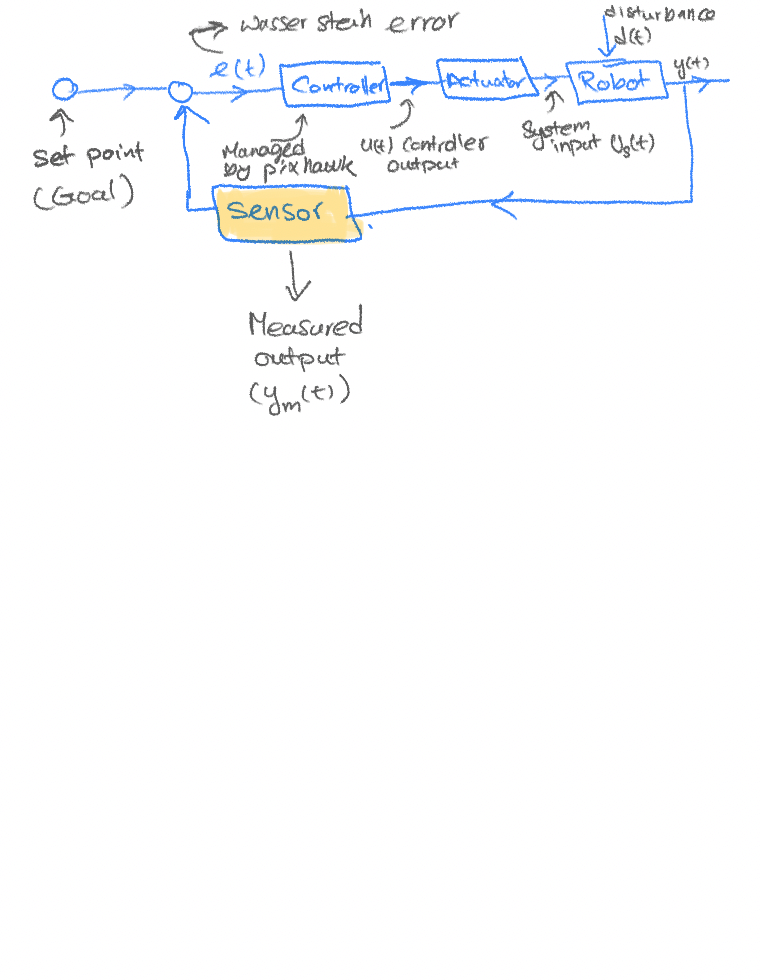
\includegraphics[width=0.9\textwidth]{controller.png}
   \end{figure}

   \begin{figure}[H]
      \centering
      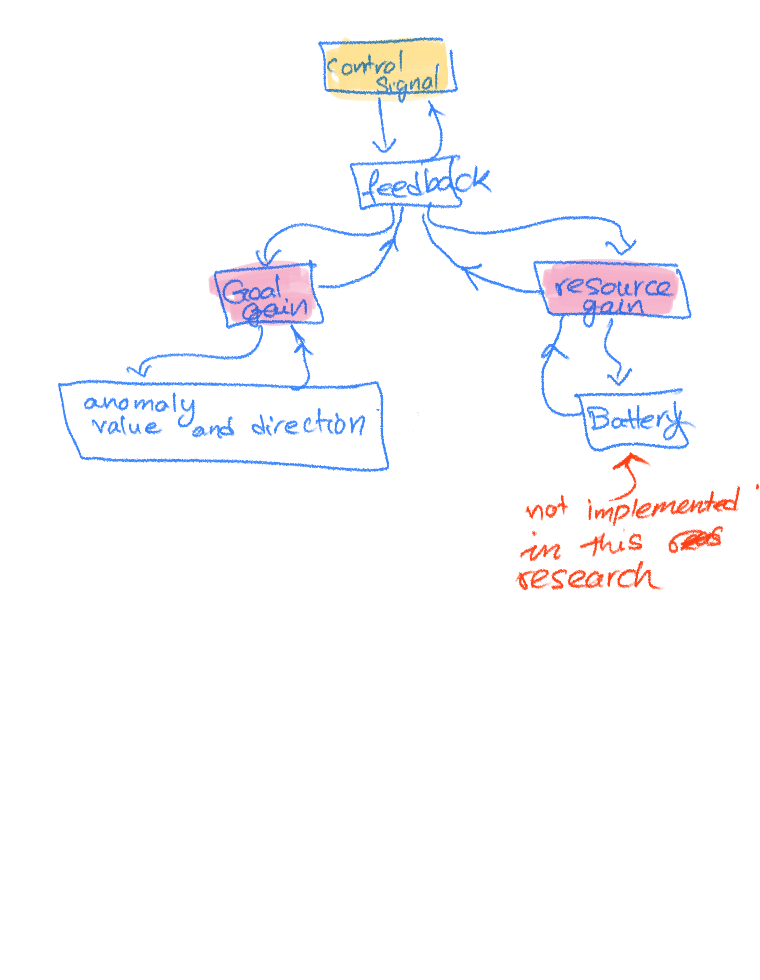
\includegraphics[width=0.9\textwidth]{feedback.png}
   \end{figure}

   \section{Cost function}
      The cost function in model predictive controller (MPC)

      for specfications \seeherefooter{https://github.com/donkarlo/nd_robotic_ai_learning_project/blob/main/src/control_theory/kind/model_predictive_control/model_predictive_control.tex}

      \begin{figure}[H]
         \centering
         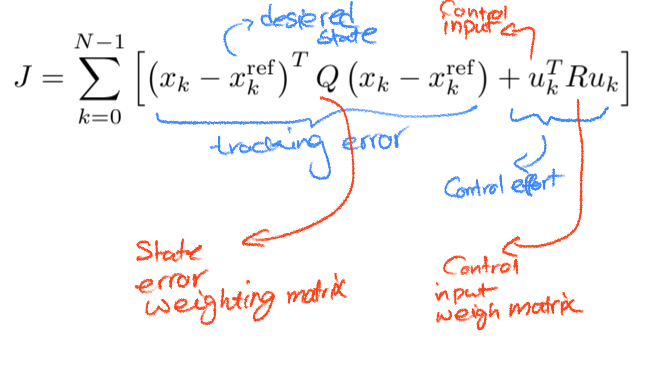
\includegraphics[width=0.9\textwidth]{cost_function}
      \end{figure}


      \begin{figure}[H]
         \centering
         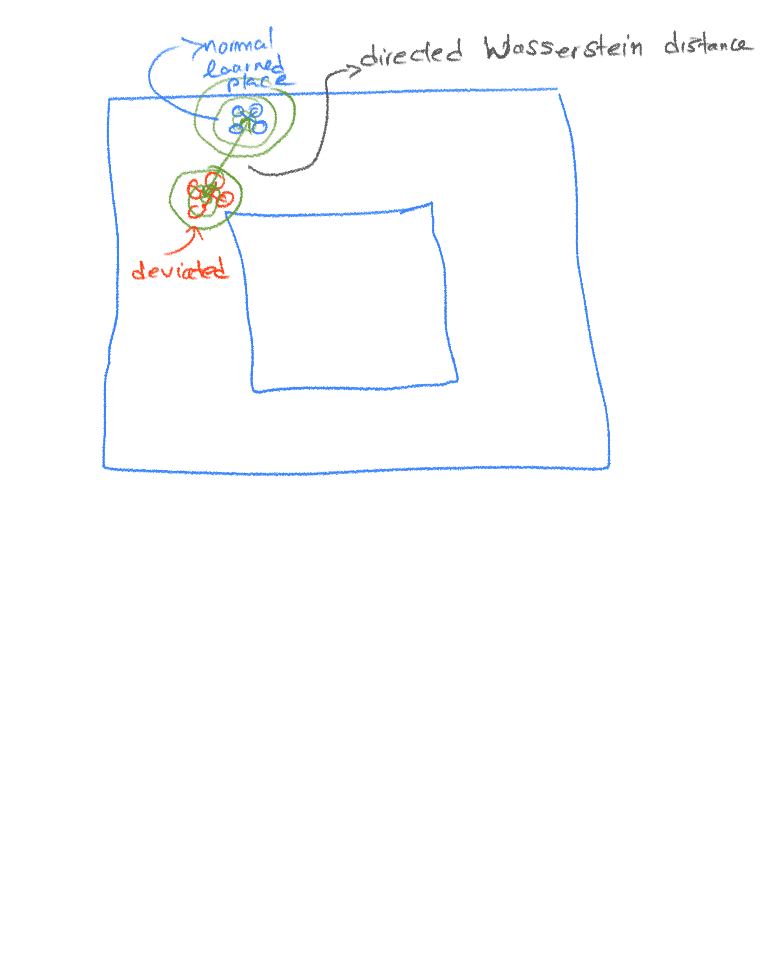
\includegraphics[width=0.9\textwidth]{autonomous_using_cost_function.png}
      \end{figure}

      \bibliographystyle{plainnat}
      \bibliography{/home/donkarlo/Dropbox/repo/nd_shared_research/bibliography/bibliography.bib}
\end{document}
